\documentclass[12pt, a4paper]{article}
\usepackage[lmargin =0.5 in,
rmargin=0.5in,
tmargin=1in,
bmargin=0.5in]{geometry}
\geometry{letterpaper}
\usepackage{tikz-cd}
\usepackage{amsmath}
\usepackage{amssymb}
\usepackage{blindtext}
\usepackage{titlesec}
\usepackage{enumitem}
\usepackage{fancyhdr}
\usepackage{amsthm}
\usepackage{graphicx}
\usepackage{cool}
\usepackage{thmtools}
\usepackage{hyperref}
\graphicspath{ }   				 %path to an image

%-------- sexy font ------------%
%\usepackage{libertine}
%\usepackage{libertinust1math}

%\usepackage{mlmodern}   			 % very nice and classic
%\usepackage[utopia]{mathdesign}
%\usepackage[T1]{fontenc}


\usepackage{mlmodern}
\usepackage{eulervm}
%\usepackage{tgtermes}    			 %times new roman
%-------- sexy font ------------%


% Problem Styles
%====================================================================%


\newtheorem{problem}{Problem}


\theoremstyle{definition}
\newtheorem{thm}{Theorem}
\newtheorem{lemma}{Lemma}
\newtheorem{prop}{Proposition}
\newtheorem{cor}{Corollary}
\newtheorem{fact}{Fact}
\newtheorem{defn}{Definition}
\newtheorem{example}{Example}
\newtheorem{question}{Question}

\newtheorem{manualprobleminner}{Problem}

\newenvironment{manualproblem}[1]{%
	\renewcommand\themanualprobleminner{#1}%
	\manualprobleminner
}{\endmanualprobleminner}

\newcommand{\penum}{ \begin{enumerate}[label=\bf(\alph*), leftmargin=0pt]}
	\newcommand{\epenum}{ \end{enumerate} }

% Math fonts shortcuts
%====================================================================%

\newcommand{\ring}{\mathcal{R}}
\newcommand{\N}{\mathbb{N}}                       	% Natural numbers
\newcommand{\Z}{\mathbb{Z}}                       	% Integers
\newcommand{\R}{\mathbb{R}}                       	% Real numbers
\newcommand{\C}{\mathbb{C}}                       	% Complex numbers
\newcommand{\F}{\mathbb{F}}                       	% Arbitrary field
\newcommand{\Q}{\mathbb{Q}}                       	% Arbitrary field
\newcommand{\PP}{\mathcal{P}}                     	% Partition
\newcommand{\M}{\mathcal{M}}                     	% Mathcal M
\newcommand{\eL}{\mathcal{L}}                     	% Mathcal L
\newcommand{\T}{\mathbb{T}}                     	% Mathcal T
\newcommand{\U}{\mathcal{U}}                     	% Mathcal U\\
\newcommand{\V}{\mathcal{V}}                     	% Mathcal V

% symbol shortcuts
%====================================================================%

\newcommand{\bd}{\partial}
\newcommand{\grad}{\nabla}
\newcommand{\lam}{\lambda}
\newcommand{\imp}{\implies}
\newcommand{\all}{\forall}
\newcommand{\exs}{\exists}
\newcommand{\delt}{\delta}
\newcommand{\ep}{\varepsilon}
\newcommand{\ra}{\rightarrow}
\newcommand{\vph}{\varphi}

\newcommand{\ol}{\overline}
\newcommand{\f}{\frac}
\newcommand{\lf}{\lfrac}
\newcommand{\df}{\dfrac}

% bracketting shortcuts
%====================================================================%
\newcommand{\abs}[1]{\left| #1 \right|}
\newcommand{\babs}[1]{\Big|#1\Big|}
\newcommand{\bound}{\Big|}
\newcommand{\BB}[1]{\left(#1\right)}
\newcommand{\dd}{\mathrm{d}}
\newcommand{\artanh}{\mathrm{artanh}}
\newcommand{\Med}{\mathrm{Med}}
\newcommand{\Cov}{\mathrm{Cov}}
\newcommand{\Corr}{\mathrm{Corr}}
\newcommand{\tr}{\mathrm{tr}}
\newcommand{\Range}[1]{\mathrm{range}(#1)}
\newcommand{\Null}[1]{\mathrm{null}(#1)}
\newcommand{\lan}{\langle}
\newcommand{\ran}{\rangle}
\newcommand{\norm}[1]{\left\lVert#1\right\rVert}
\newcommand{\inn}[1]{\lan#1\ran}
\newcommand{\op}[1]{\operatorname{#1}}
\newcommand{\bmat}[1]{\begin{bmatrix}#1\end{bmatrix}}
\newcommand{\pmat}[1]{\begin{pmatrix}#1\end{pmatrix}}
\newcommand{\vmat}[1]{\begin{vmatrix}#1\end{vmatrix}}

\newcommand{\amogus}{{\bigcap}\kern-0.8em\raisebox{0.3ex}{$\subset$}}
\newcommand{\Note}{\textbf{Note: }}
\newcommand{\Aside}{{\bf Aside: }}
%restriction
%\newcommand{\op}[1]{\operatorname{#1}}
%\newcommand{\done}{$$\mathcal{QED}$$}

%====================================================================%


\setlength{\parindent}{0pt} 		 % No paragraph indentations
\pagestyle{fancy}
\fancyhf{}   						 % fancy header

\setcounter{secnumdepth}{0}   		 % sections are numbered but numbers do not appear
\setcounter{tocdepth}{2}    		 % no subsubsections in toc

%template
%====================================================================%
%\begin{manualproblem}{1}
%Spivak.
%\end{manualproblem}

%\begin{proof}[Solution]
%\end{proof}

%----------- or -----------%

%\begin{problem}    	 
%\end{problem}    

%\penum
%    \item
%\epenum
%====================================================================%


\newcommand{\Course}{351}
\newcommand{\hwNumber}{7}

%preamble

\title{}
\author{A.N.}
\date{\today}
\lhead{\Course A\hwNumber}
\rhead{\thepage}
%\cfoot{\thepage}


%====================================================================%
\begin{document}
	
	
	
	\begin{problem}
	\end{problem}
	Suppose both $f$ satisfies $f^\prime(l) =cf(l), f^\prime(0) = - cf(0)$, and $g$ does as well.  We compute:
	\begin{align*}
		\left[f^\prime(x) g(x) - f(x)g^\prime(x)\right] \Big|_0^l& = f^\prime(l)g(l) - f(l)g^\prime(l)- f^\prime(0)g(0) + f(0)g^\prime(0)
		\\ & = cf(l)g(l)-cf(l)g(l)+ cf(0)g(0)- cf(0)g(0)
		\\ & = 0
	\end{align*}
	Therefore for $f,g$ with identical boundary conditions, we have that they are symmetric. This implies eigenfunctions with the same boundary conditions but different eigenvalues of $\frac{d^2}{dx^2}$ are orthogonal, and hence form an orthonormal basis of the Hilbert space.
	\newpage
	\begin{problem}
	\end{problem}
	Recall from Assignment 6 that for any $f\in C^2$ the following holds: $$c_n(f^{\prime \prime}) = \frac{-n^2}{2\pi} c_n(f).$$
	Consider now the Fourier Series of $f$, given as $\sum_{n\geq 1}e^{inx}c_n(f)$. We can bound each term of the sum in the following way:
	$$|e^{inx}c_n(f)| = \frac{2\pi}{n^2}|c_n(f^{\prime \prime})| = \frac{1}{n^2} \Big|\int_0^{2\pi } e^{inx}f(x) dx
	\Big| \leq \frac{1}{n^2} \int_0^{2\pi} |f^{\prime \prime}(x)|dx \leq \frac{2\pi \sup|f^{\prime \prime}|}{n^2}.$$
	We have that the sum $\sum_{n\geq 1} \frac{2\pi \sup |f^{\prime \prime}|}{n^2}$ converges, so by the M-Test the Fourier series of $f$ converges absolutely and uniformly.
	\newpage
	\begin{problem}
	\end{problem}
	We wish to solve the following boundary value problem:
	$$\begin{cases}
		u_{tt} = c^2u_{xx} &\text{on $(0,l)$}\\
		u(0,t) = u_t(l,t) = 0 \\
		u(x,0)=x^2\\
		u_t(x,0) = x
	\end{cases}$$
	Writing $u(x,t) = X(x)T(t)$, we know that $X,T$ take the following forms:
	$$T(t) = A_n \sin(c\lambda_n t) + B_n \cos (c \lambda_n t), X(x) = A_n^\prime \sin(\lambda_n x) + B_n^\prime \cos(\lambda_n x).$$
	We first look at $X(x)$. Note that since $X(0)=0$, we have that $B_n^\prime = 0$. Since $X^\prime(l)= \lambda_n A^\prime_n \cos(\lambda_n l) = 0$, we have that $\lambda_n = \frac{n\pi}{l} + \frac{\pi}{2l}$. So $$X(x) = A_n^\prime \sin \left(\left(\frac{n\pi}{l} + \frac{\pi}{2l}\right)x \right).$$
	
	Thus we write $$u(x,t) = \sum_{n\geq 1} \left(A_n\sin \left(ct \left(\frac{n\pi}{l} + \frac{\pi}{2l}\right) \right) + B_n \cos \left( ct\left(\frac{n\pi}{l} + \frac{\pi}{2l} \right) \right)  \right)\sin \left(x \left(\frac{n\pi}{l} + \frac{\pi}{2l}\right) \right)$$
	Now using the initial conditions we have that
	$$\begin{cases}
		u(x,0) = x^2 = \sum B_n\sin \left(x \left(\frac{n\pi}{l} + \frac{\pi}{2l}\right) \right) \\
		u_t(x,0) = x = \sum A_n \cdot c  \cdot (\frac{n\pi}{l} + \frac{\pi}{2l}) \sin \left(x \left(\frac{n\pi}{l} + \frac{\pi}{2l}\right) \right).
	\end{cases}$$
	Orthongonality of the basis implies that $$B_n = \frac{2}{l} \int_0^l x^2 \sin \left(x \left(\frac{n\pi}{l} + \frac{\pi}{2l}\right) \right) dx = \frac{(-1)^n \cdot 4l^2 \cdot (8\pi n + 4\pi n)}{\pi^3(2n+1)^3} = \frac{(-1)^n 16l^2 }{\pi^2 (2n+1)^2}.$$
	Similarly for the $A_n's$, we have that
	$$A_n = \frac{1}{c} \cdot \frac{2}{l} \cdot \frac{1}{\frac{n\pi}{l} + \frac{\pi}{2l}} \cdot \frac{(-1)^n 4l^3}{\pi^2 (2n+1)^2} = \frac{(-1)^n 16l^3}{c\pi^3(2n+1)^3}$$
	\newpage
	\begin{problem}
	\end{problem}
	First for $f_n = x^n$ on $[0,1]$, pointwise this does not converge to a continuous function. It converges to $\delta_1(x)$.
	Furthermore it does not converge uniformly, since it does not converge pointwise. We claim that it converges to $0$ in $L^2$ however. Observe:
	$$\int_0^1 |x^n|^2 dx = \int_0^1 x^{2n}dx = \frac{1}{2n+1},$$
	which goes to 0 as $n \to \infty$.
	Now for $g_n(x) = nx^n$. This does not converge pointwise or uniformly since $g_n(1) \to \infty$ as $n \to \infty$. We now verify if $g_n(x)$ converges in $L^2$:
	$$\int_0^1 |nx^n|^2 dx = \int_0^1 n^2 x^{2n}dx = \frac{n^2}{2n+1},$$
	which diverges in $L^2$.
	The following picture demonstrates a family of functions which converge to $0$ pointwise, but does not converge to $0$ in $L^2$.
	$$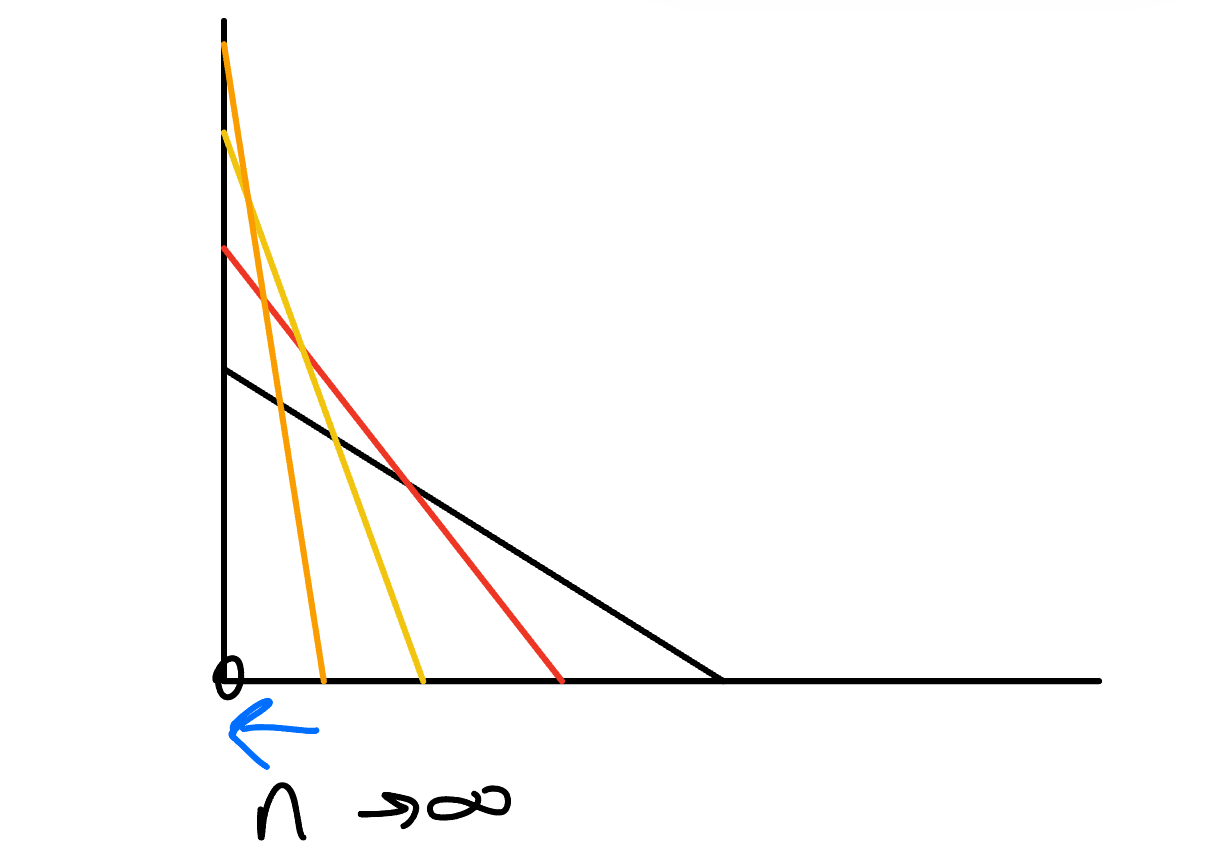
\includegraphics[width=0.5\textwidth]{A7Q4.png}.$$
	where the functions are normalized so that their integral is $1$. The converse is not true. Suppose we have a family of functions $\{f_n\}$ which converge to $0$ in $L^2$. We have that $\int_0^1 |f_n|^2 dx \to 0.$ This means that $|f_n|^2 \to 0$ almost everywhere, and so $f_n \to 0$ almost everywhere.
	\newpage
	\begin{problem}
	\end{problem}
	\penum
	\item Recall that it has been computed in Lectures that the Fourier sin series of $\phi(x) = x$ on $(0,l)$ is
	$$\phi(x) = \sum_n (-1)^{n+1}\frac{ 2l}{n\pi} \sin \frac{n\pi x}{l}.$$
	Since $x^2 = 2 \int_0^x y dy$, we can easily obtain the Fourier cosine series of $x^2$ by integrating $\phi(x)$ term by term.
	So,
	\begin{align*}
		x^2 &= A_0+ 2 \int_0^x\sum_n (-1)^{n+1}\frac{ 2l}{n\pi} \sin \frac{n\pi y}{l} dy
		\\ & = A_0 + \sum_n (-1)^{n+1} \frac{4l}{n\pi} \int_0^x \sin \frac{n\pi y}{l} dy
		\\ & =  A_0 +  \sum_n (-1)^{n} \frac{4l^2}{n^2\pi^2} \cos\frac{n\pi x}{l}
	\end{align*}
	Where $A_0 = \frac{1}{l} \int_0^l x^2 dx  = \frac{1}{3}l^2$. At $x=0$, the above gives us:
	$$\frac{1}{3}l^2 = \sum_n (-1)^{n+1}\frac{4l^2}{n^2\pi^2} \implies \sum \frac{(-1)^{n+1}}{n^2} =\frac{\pi^2}{12} $$
	\item We now determine the Fourier series of $x^3,x^4$ in the same way. We first find the sin series of $x^3$. We have that 4
	$$x^3 = \sum_{n\geq 1} A_n \sin \frac{n\pi x}{l}.$$
	Orthogonality tells us that
	$$A_n = \frac{2}{l} \int_0^l  x^3 \sin\frac{n\pi x}{l} = \frac{2l^3 (-1)^{n+1}}{\pi n} - \frac{12l^3(-1)^{n+1}}{\pi^3 n^3}.$$
	Therefore $$x^3 = \sum_{n\geq 1}\left(\frac{2l^3 (-1)^{n+1}}{\pi n} - \frac{12l^3(-1)^{n+1}}{\pi^3 n^3} \right) \sin \frac{x\pi n}{l}.$$
	We perform the same trick as above to obtain the Fourier series for $x^4$, integrating. We have that $$x^4 = A_0+ 4\int_0^x y^3 dy$$ with $$A_0= \frac{1}{2l} \int_0^l x^4 =  \frac{l^4}{10}.$$
	Therefore
	\begin{align*}
		x^4 &= \frac{l^4}{10} + 4\int_0^x y^3 dy
		\\ & = \frac{l^4}{10} +4 \int_0^x \sum_{n\geq 1} A_n \sin \frac{n\pi y}{l} dy
		\\ & = \frac{l^4}{10} + 4\sum_{n\geq 1} A_n \int_{0}^x \sin \frac{n\pi y}{l} dy
		\\ & = \frac{l^4}{10} +4 \sum_{n\geq 1} A_n \frac{l}{n \pi} \cdot -\cos \frac{n\pi x}{l}
	\end{align*}
	\item At $x = 0$, we have that
	$$0 = \frac{l^4}{10} +4 \sum_{n\geq 1} A_n \frac{l}{n \pi} = \frac{l^4}{10} + 4\sum_{n \geq 1}\frac{2l^4 (-1)^{n+1}}{\pi^2 n^2} - \frac{12l^4(-1)^{n+1}}{\pi^4 n^4} \implies \frac{\pi^4}{45} = \sum_{n\geq 1}\frac{(-1)^n}{n^4}$$
	%test test test
	\epenum
\end{document}


